% !TeX root = ../main.tex
% Add the above to each chapter to make compiling the PDF easier in some editors.

\chapter{Introduction}\label{chapter:introduction}
Cloud computing moves towards smaller deliverables. First hardware, then infrastructure, virtual machines, platforms, containers, and functions. While customers are facing with smaller deliverables, the background stays mostly the same. Even if the user only deploys a function, cloud provider creates an OS and deploys a containerized application that runs the given user function. There are at least 3 different abstractions between what user wants to run (their function) and where it runs ( hardware). That's 2 times more than the desired abstraction level. There should be a way to decrease the distance between the hardware and the user application without compromising the flexibility of cloud computing. 
\begin{figure}[htpb]
  \centering
  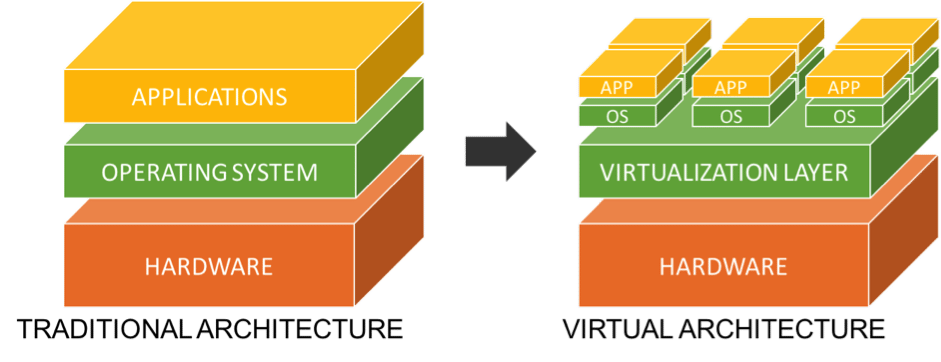
\includegraphics[width=0.8\textwidth]{figures/1-123.png}
  \caption{Moving from traditional architecture to virtualization based architecture: \cite{arch-photo} } \label{fig:arch}
\end{figure}
\section{Motivation}
Unikernels are special programs that package application code together with a minimal operating system image.\cite{7396164} These special programs can be booted like operating systems and more interestingly , they can also be virtualized like operating systems. That means we can do , in theory, any scheduling operation we normally do on virtual machines with unikernels. In the current landscape of orchestration technologies , this opens up many new improvements to apply the principles of deployment, scaling and scheduling to a new domain.

Kubernetes is an open source project for automating orchestration of containerized applications. \cite{Hightower:2017:KUR:3175917} Kubernetes by default uses Docker as it's runtime. Both It's own components and user defined components are deployed as docker containers. Instead of giving commands to virtual machines separately with projects such as Puppet or Ansible, all those virtual machines are connected in a Kubernetes cluster and user only interacts with the Kubernetes API which schedules deployments according to the rules and requirements.

The Docker runtime requires a host operating system to run the Docker daemon, so this requires every node to have a complete operating system to run even simple applications. Those operating systems also run background jobs that come with the OS but not required by the running applications. E.g. a USB driver or a sound driver is not vital for a web server but the operating system still runs them by default. Because of this drawback, there is a new branch of operating systems, like container linux (previously coreos)\cite{coreos}, where the OS is optimized to run only containers. Nevertheless for an ephemeral web server which only answer requests with static data embedded inside the container, the OS still has to run a filesystem. There is no requirements agreement between OS and the application running on top of it.

A fairly new techology, called Unikernel, compiles an OS with only functions required by the compiled application logic. E.g. If a program doesn't require networking, the networking stack is not included in the final image. That creates a much smaller artifact which can be booted directly by hypervisors as It's actually an OS in practice. It has many advantages over the Docker runtime. As a start, It decreases the "scaling time \cite{Podolskiy:2017:QCA:3069383.3069390}" of the applications; because, first no operating system is required to boot up, and second the applications are much more smaller , so they can be downloaded faster.

The proposed effects of a Kubernetes cluster running together with a unikernel extension can be summarised as follows:

\subsection{Security}
 The host OS's are required for the multi-tenant cloud architecture to achieve isolation. Otherwise, vulnerability in one of the containers could compromise all other containers running on the same VM. On the other hand, a vulnerability found in the operating system can also compromise the running applications. With Unikernel, the operating system consists only by the application, there is no other attack surface. Even if the unikernel program gets compromised, the hypervisor underneath will prevent other programs from compromising too.

\subsection{Resource Utilization}
The user never interacts with the underlying operating system that their application is running on. It is only used by the cloud provider infrastructure. Despite that, the user still pays for the resources used by the operating system. Unikernels remove the container level abstraction and combine It with VM abstraction. Users only pay for what their application uses as there is nothing else to pay for and because they VMs only run their applications they don't pay for CPU cycles used by background jobs of an OS.

\subsection{Scaling Time}
Unikernels have a very small footprint and can run on hardwares through a hypervisor. This makes much faster boot up times possible which in combination with scalability, improves the current status quo of scalability metrics. It's on demand design allows scalability ideas to be used in scenarios which were not available before, such as inside DNS servers.

\subsection{IoT Scenarios}
Unikernels also have role in the IoT world. Their size allows them to be deployed to places with sparse internet connection or low-end devices. Their security story makes them hard targets in the IoT ecosystem, where security practices are still a challenge for developers\cite{iot-sec}. They can be configured to read data from the host devices they are running on , with fine grained access control. Kubernetes can be used to schedule them to IoT devices. Kubernetes comes in handy for such scenarios, because users can label their deployments and Kubernetes will deploy them to respective devices. Multiple unikernel applications can be deployed to the same device with a single deployment through the Kubernetes API. Given that multiple unikernels can run on the same device, a microservice based architecture can also be used for IoT programs where a single unikernel is tasked with only one job and it communicates with other unikernels through a shared medium locally on the device or through Kubernetes services. This allows distributed computing paradigms to be used on IoT devices with Kubernetes orchestrating it.

